\documentclass[a4paper]{article}
\usepackage{geometry}
\usepackage{graphicx}
\usepackage{natbib}
\usepackage{amsmath}
\usepackage{amssymb}
\usepackage{amsthm}
\usepackage{paralist}
\usepackage{epstopdf}
\usepackage{tabularx}
\usepackage{longtable}
\usepackage{multirow}
\usepackage{multicol}
\usepackage[hidelinks]{hyperref}
\usepackage{fancyvrb}
\usepackage{algorithm}
\usepackage{algorithmic}
\usepackage{float}
\usepackage{paralist}
\usepackage[svgname]{xcolor}
\usepackage{enumerate}
\usepackage{array}
\usepackage{times}
\usepackage{url}
\usepackage{fancyhdr}
\usepackage{comment}
\usepackage{environ}
\usepackage{times}
\usepackage{textcomp}
\usepackage{caption}


\urlstyle{rm}

\setlength\parindent{0pt} % Removes all indentation from paragraphs
\theoremstyle{definition}
\newtheorem{definition}{Definition}[]
\newtheorem{conjecture}{Conjecture}[]
\newtheorem{example}{Example}[]
\newtheorem{theorem}{Theorem}[]
\newtheorem{lemma}{Lemma}
\newtheorem{proposition}{Proposition}
\newtheorem{corollary}{Corollary}

\floatname{algorithm}{Procedure}
\renewcommand{\algorithmicrequire}{\textbf{Input:}}
\renewcommand{\algorithmicensure}{\textbf{Output:}}
\newcommand{\abs}[1]{\lvert#1\rvert}
\newcommand{\norm}[1]{\lVert#1\rVert}
\newcommand{\RR}{\mathbb{R}}
\newcommand{\CC}{\mathbb{C}}
\newcommand{\Nat}{\mathbb{N}}
\newcommand{\br}[1]{\{#1\}}
\DeclareMathOperator*{\argmin}{arg\,min}
\DeclareMathOperator*{\argmax}{arg\,max}
\renewcommand{\qedsymbol}{$\blacksquare$}

\definecolor{dkgreen}{rgb}{0,0.6,0}
\definecolor{gray}{rgb}{0.5,0.5,0.5}
\definecolor{mauve}{rgb}{0.58,0,0.82}

\newcommand{\Var}{\mathrm{Var}}
\newcommand{\Cov}{\mathrm{Cov}}

\newcommand{\vc}[1]{\boldsymbol{#1}}
\newcommand{\xv}{\vc{x}}
\newcommand{\Sigmav}{\vc{\Sigma}}
\newcommand{\alphav}{\vc{\alpha}}
\newcommand{\muv}{\vc{\mu}}

\newcommand{\red}[1]{\textcolor{red}{#1}}

\def\x{\mathbf x}
\def\y{\mathbf y}
\def\w{\mathbf w}
\def\v{\mathbf v}
\def\E{\mathbb E}
\def\V{\mathbb V}

% TO SHOW SOLUTIONS, include following (else comment out):
\newenvironment{soln}{
    \leavevmode\color{blue}\ignorespaces
}{}


\hypersetup{
%    colorlinks,
    linkcolor={red!50!black},
    citecolor={blue!50!black},
    urlcolor={blue!80!black}
}

\geometry{
  top=1in,            % <-- you want to adjust this
  inner=1in,
  outer=1in,
  bottom=1in,
  headheight=3em,       % <-- and this
  headsep=2em,          % <-- and this
  footskip=3em,
}


\pagestyle{fancyplain}
\lhead{\fancyplain{}{Homework 3}}
\rhead{\fancyplain{}{CS 760 Machine Learning}}
\cfoot{\thepage}

\title{\textsc{Homework 3}} % Title

%%% NOTE:  Replace 'NAME HERE' etc., and delete any "\red{}" wrappers (so it won't show up as red)

\author{
\red{$AKASH SHARMA$} \\
\red{$9081731771$}\\
} 

\date{}

\begin{document}

\maketitle 


\textbf{Instructions:} 
Although this is a programming homework, you only need to hand in a pdf answer file.
There is no need to submit the latex source or any code.
You can choose any programming language, as long as you implement the algorithm from scratch. 

Use this latex file as a template to develop your homework.
Submit your homework on time as a single pdf file to Canvas.
Please check Piazza for updates about the homework.

\section{A Simplified 1NN Classifier}
You are to implement a 1-nearest-neighbor learner for classification.
To simplify your work, your program can assume that
\begin{itemize}
\item each item has $d$ continuous features $\x \in \RR^d$
\item binary classification and the class label is encoded as $y \in \{0,1\}$
\item data files are in plaintext with one labeled item per line, separated by whitespace:
$$x_{11} \quad \ldots \quad x_{1d} \quad y_1$$
$$...$$
$$x_{n1} \quad \ldots \quad x_{nd} \quad y_n$$
\end{itemize}

Your program should implement a 1NN classifier: 
\begin{itemize}
\item Use Mahalanobis distance $d_A$ parametrized by a positive semidefinite (PSD) diagonal matrix $A$.  For $\x, \x' \in \RR^d$,
$$d_A(\x,\x') = \|\x-\x'\|_A = \sqrt{(\x-x')^\top A (\x-x')}.$$
We will specify $A$ in the questions below. (Hint: $d$ is dimension while $d_A$ with a subscript is distance)
\item If multiple training points are the equidistant nearest neighbors of a test point, you may use any one of those training points to predict the label.
\item You do not have to implement kd-tree.
\end{itemize}

\section{Questions}
\begin{enumerate}

\item (5 pts) What is the mathematical condition on the diagonal elements for a diagonal matrix $A$ to be PSD?
\begin{soln}
For a diagonal matrix A to be a positive semidefinite diagonal matrix, the eigen values of A must be greater than or equal to 0. Since, the eigen values of the diagonal matrix conincide with the diagonal entries, the diagonal elements of the diagonal matrix must be greater than or equal to 0.
\end{soln}

\item (5 pts) Given a training data set $D$, how do we preprocess it to make each feature dimension mean 0 and variance 1? (Hint: give the formula for $\hat \mu_j, \hat \sigma_j$ for each dimension $j$, and explain how to use them to normalize the data.  You may use either the $1 \over n$ or $1 \over n-1$ version of sample variance.  You may assume the sample variances are non-zero.) 
\begin{soln}
\\We can preprocess the data by subtracting the mean of each feature (all feature values from the dataset) from the feature value, and dividing by the respective variance of each feature as well. 
\end{soln}

\item (5 pts) Let $\tilde \x$ be the preprocessed data. Give the formula for the Euclidean distance between $\tilde \x, \tilde \x'$.
\begin{soln}
	\\Since, $\tilde \x$ is the preprocessed data, each of the values of the original dataset is normalized, that is, the mean is subtracted, and values are divided by the standard deviation of each feature.
	$$Euclidean(\tilde \x,\tilde \x') = \sqrt{\sum_{i}(\tilde \x_{i}-\tilde \x'_{i})^2}$$
	\\Here, each value of feature $\tilde \x_{i}$ is,  $$(x_{i} - \mu_{i})/\sigma_{i} $$  where  $  \x_{i} $ is the original feature, $ \mu_{i} $  is the mean, and  $ \sigma_{i} $  is the standard deviation of the $i_{th}$ feature.  
\end{soln}

\item (5 pts) Give the equivalent Mahalanobis distance on the original data $\x, \x'$ by specifying $A$. (Hint: you may need $\hat \mu_j, \hat \sigma_j$)
\begin{soln}
 \\The equivalent Mahalonobis distance can be calculated as below: 
	$$d_A(\x,\x') = \|\x-\x'\|_A = \sqrt{(\x-x')^\top A (\x-x')}.$$
	where 	
	\[
A=
  \begin{bmatrix}
    a_{11} & 0 & 0 & \dots  & 0 \\
    0 & a_{22} & 0 & \dots  & 0 \\
    \vdots & \vdots & \vdots & \ddots & \vdots \\
    0 & 0 & 0 & \dots  & a_{dd}
  \end{bmatrix}
\]

Putting the value of A in the above equation and mutiplying the matrices, we get 
$$ A = \sqrt{\sum_{i}a_{ii}( x_{i}- x'_{i})^2}$$

Now, comparing this with the above Euclidean distance,

	$$Euclidean(\tilde \x,\tilde \x') = \sqrt{\sum_{i}(\tilde \x_{i}-\tilde \x'_{i})^2}$$
Here, each value of feature $\tilde \x_{i}$ is,  $$(x_{i} - \mu_{i})/\sigma_{i} $$  where  $  \x_{i} $ is the original feature, $ \mu_{i} $  is the mean, and  $ \sigma_{i} $  is the standard deviation of the $i_{th}$ feature.
\\Replacing the value of $\tilde \x_{i}$, that is,  $$(x_{i} - \mu_{i})/\sigma_{i} $$ above we get,  $$\sqrt{\sum_{i} 1/(\sigma_{i})^{2}( \x_{i}- \x'_{i})^2}$$

Therefore, on comparing the equations above, the PSD matrix must have each of its Diagonal values as $1/\sigma_{i}^{2}$. 
The equivalent Mahalonobis distance is 
$$d_A(\x,\x') = \|\x-\x'\|_A = \sqrt{(\x-x')^\top A (\x-x')}$$, 
where

\[
	A=
  \begin{bmatrix}
    1/(\sigma_{1})^{2} & 0 & 0 & \dots  & 0 \\
    0 & 1/(\sigma_{2})^{2} & 0 & \dots  & 0 \\
    \vdots & \vdots & \vdots & \ddots & \vdots \\
    0 & 0 & 0 & \dots  & 1/(\sigma_{d})^{2}
  \end{bmatrix}
\]

\end{soln}

\item (5 pts) Let the diagonal elements of $A$ be $a_{11}, \ldots, a_{dd}$.
Define a diagonal matrix $L$ with diagonal $\sqrt{a_{11}}, \ldots, \sqrt{a_{dd}}$.
Define $\tilde \x = L\x$.
Prove that $d_I(\tilde \x, \tilde \x') = d_A(\x, \x')$ where $I$ is the identity matrix.

\begin{soln}
As L is a diagonal matrix with diagonal $\sqrt{a_{11}}, \ldots, \sqrt{a_{dd}}$,

	\[
L=
  \begin{bmatrix}
    \sqrt{a_{11}} & 0 & 0 & \dots  & 0 \\
    0 & \sqrt{a_{22}} & 0 & \dots  & 0 \\
    \vdots & \vdots & \vdots & \ddots & \vdots \\
    0 & 0 & 0 & \dots  & \sqrt{a_{dd}}
  \end{bmatrix}
\]

 As, $\tilde \x = L\x $, so 
\[
\tilde \x=
  \begin{bmatrix}
    \sqrt{a_{11}}x_{1} \\
    \sqrt{a_{22}}x_{2} \\
    \vdots \\
    \sqrt{a_{dd}}x_{d}
  \end{bmatrix}
\]

$d_I(\tilde \x, \tilde \x')  = \sqrt{(\tilde \x-\tilde \x')^\top A (\tilde \x-\tilde \x')} $ 
\\Since, A = Identity, 
$d_I(\tilde \x, \tilde \x')  = \sqrt{(\tilde \x-\tilde \x')^\top (\tilde \x-\tilde \x')} =  \sqrt{\sum_{i}a_{ii}( x_{i}- x'_{i})^2} $

Looking at the RHS of the equation, 
$$d_A(\x,\x')  = \sqrt{(\x-x')^\top A (\x-x')}$$
\[
A=
  \begin{bmatrix}
    a_{11} & 0 & 0 & \dots  & 0 \\
    0 & a_{22} & 0 & \dots  & 0 \\
    \vdots & \vdots & \vdots & \ddots & \vdots \\
    0 & 0 & 0 & \dots  & a_{dd}
  \end{bmatrix}
\]

the values of L are the square root of those in A. On expanding the above, we get  LHS = RHS = $\sqrt{\sum_{i}a_{ii}( x_{i}- x'_{i})^2} $. Hence LHS = RHS.

\end{soln}

\item (5 pts) Geometrically, what does $L\x$ do to the point $\x$?  Explain in simple English.
\begin{soln}
	\\The Matrix L when multiplied with x, results in increasing or decreasing the values of each feature of x, resulting it to move in the feature space.
\end{soln}

\item (10 pts) Let $U$ be any orthogonal matrix.
Define $\tilde \x = UL\x$. 
\\(i) Prove that $d_I(\tilde \x, \tilde \x') = d_A(\x, \x')$ again. 
\begin{soln}
\\Since, U is an Orthogonal Matrix, $U_{T}U = I $.
Expanding the LHS with A = I, and $\tilde \x = UL\x$

$d_I(\tilde \x, \tilde \x')  = \sqrt{(\tilde \x-\tilde \x')^\top (\tilde \x-\tilde \x')} = \sqrt{( UL\x - UL\x')^\top (UL\x - UL\x')}$
\\$d_I(\tilde \x, \tilde \x')  = \sqrt{(UL)^{T}( \x - \x')^\top UL (\x - \x')}$
\\Using the property, $(UL)^{T} = L^{T}U^{T}$
, and using the Orthogonal property, $U^{T}U = I $, and $L^{T}L = L^{2}$ in the equation below we get,
\\$d_I(\tilde \x, \tilde \x')  = \sqrt{( \x - \x')^\top L^{2} (\x - \x')}$
Since, $L^{2} = A$, we get 
\\$d_I(\tilde \x, \tilde \x') = d_A(\x, \x')$
\end{soln}

(ii) Geometrically, what does $UL\x$ do to the point $\x$?  Explain in simple English.
\begin{soln}
\\$UL\x$ when multiplied to a point $\x$ results in the linear transformation of the vector, such as rotation, reflection or rotoreflection. Its a unitary transformation.

\end{soln}

\item (20 pts) Use the whole D2z.txt as training set.  Use Euclidean distance (i.e. $A=I$).
Visualize the predictions of 1NN on a 2D grid $[-2:0.1:2]^2$.
That is, you should produce test points whose first feature goes over $-2, -1.9, -1.8, \ldots, 1.9, 2$, so does the second feature independent of the first feature.
You should overlay the training set in the plot, just make sure we can tell which points are training, which are grid.

\begin{soln}
The plot below shows the grid (test set) and the training set along with the labels. Here, red denotes the points with label 0 in the training set, while yellow denotes the points with label 1 in the training set (D2z.txt). While, green denotes the points with label 0 in the testing set, and blue denotes the points with label 1 in the testing set.

\begin{figure}[h!]
	        \centering
	        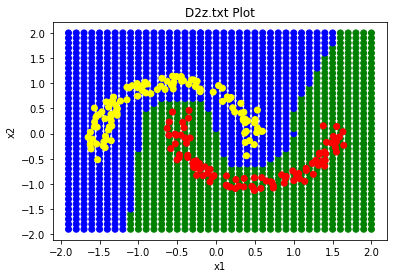
\includegraphics[width=0.6\textwidth]{D2zPlot.png} 
	        \captionsetup{labelformat=empty}
	        \caption{D2z Scatter Plot}
	        \label{fig:D2z Scatter Plot}
	   \end{figure}
\end{soln}

\item (To normalize, or not to normalize?)
Start from D2a.txt.  Perform 5-fold cross validation.
  \begin{enumerate}
  \item (5 pts) Do not normalize the data.  Report 1NN cross validation error rate for each fold, then the average (that's 6 numbers).

\begin{soln}		
	For, D2a.txt, without normalizing the data, the 1NN cross validation error rate is 0. The values for each fold is: [0.0, 0.0, 0.0, 0.0, 0.0]. The average 1NN cross validation error rate is also 0. 	
\end{soln} 

  \item (5 pts) Normalize the data.  Report 1NN cross validation error rate (again 6 numbers).  (Hints: Do not normalize the labels!  The relevant quantities should be estimated from the training portion, but applied to both training and validation portions.  This should happen 5 times.  Also, you would either change $\x$ into $\tilde    \x = L\x$ but then use Euclidean distance on $\tilde \x$, or do not change $\x$ but use an appropriate $A$; don't mix the two.)
\begin{soln}		
\\For, D2a.txt, after normalizing the data, the values for each fold is: [0.13, 0.06, 0.1, 0.17, 0.08]. The average 1NN cross validation error rate is 0.108. 	
\end{soln}  


\item (5 pts) Look at D2a.txt, explain the effect of normalization on CV error.  Hint: the first 4 features are different than the next 2 features.
\begin{soln} 
	\\After Normalizing the dataset, the cross validation error is increasing for D2a.txt. In this dataset, all features are not contributing equally to the classification of labels. The scales of the features are also different. So, when we normalise the data, the scales become same for all the features and now are contributing equally.   
\end{soln} 

  \end{enumerate}


\item (Again.  10 pts)
Repeat the above question, starting from D2b.txt.
\begin{soln}
	\\(a) For, D2b.txt, without normalizing the data, the values for each fold is: [0.16, 0.18, 0.15, 0.28, 0.17]. The average 1NN cross validation error rate is 0.188.
	\\\\(b) For, D2b.txt, after normalizing the data, the values for each fold becomes 0, that is: [0.0, 0.0, 0.0, 0.0, 0.0]. The average 1NN cross validation error rate is also 0.0.
	\\\\(c) After Normalizing the dataset, the cross validation error is decreasing for D2b.txt. In this dataset, before normalisation all features are not contributing equally to the classification of labels. The scales of the lables are also different. So, when we normalise the data, the scales become same for all values and now are contributing equally, which is favourable in this case, as the error is decreasing.
\end{soln}

\item (5 pts) What do you learn from Q9 and Q10?
\begin{soln}
	\\So, in Q9 and Q10, we see different effects of normalisation on the cross validation error. In Q9, after normalisation, the error is increasing, and in Q10, it is decreasing. So, we can say that normalisation always won't lead to a decrease in cross validation errors. In certain datasets, the output might depend more on one of the features, while it might depend less on other features. So, if we normalise the dataset, it will scale all features equally, which might lead to an increase or decrease in cross validation errors.    
\end{soln}

\item (Weka, 10 pts)
Repeat Q9 and Q10 with Weka.
Convert appropriate data files into ARFF format.
Choose classifiers / lazy / IBk.
Set $K=1$.
Choose 5-fold cross validation.
Let us know what else you needed to set.  Compare Weka's results to your Q9 and Q10.
\begin{soln}
	\\For this question, we also had to set the values of normalise parameter to True or False, and had to keep the K values as 1, and fold value as 5.
	\\For D2a.txt, the value for cross validation error without normalisation is 0. After normalisation, the value of cross validation becomes 0.06. So, this value is lower as compared to my cross validation error computed in Q9. 
	\\For D2b.txt, the value for cross validation error after normalisation is 0. Before normalisation, the value of cross validation error is 0.10.

\end{soln}

\end{enumerate}

\bibliographystyle{apalike}
\end{document}
